\subsection{Modelo}

Recordemos que el objetivo principal del acceso a los datos, es obtener conocimiento. Hay que tener en 
cuenta que los datos por si solos, no tienen ningun valor, ya que carecen de sentido, una vez integrados en un contexto,
nos aportara informacion, y procesando y analizando esta informacion, se obtendra el conocimiento.\\
    
\begin{figure}[ht]
    \centering 
    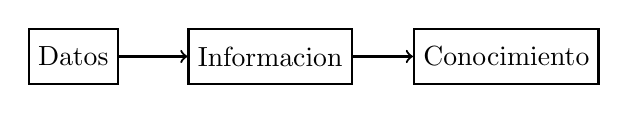
\begin{tikzpicture}[thick]
        \node[draw,rectangle,minimum size=20] (a) {Datos};
         \node[draw,rectangle,minimum size=20,right of= a, node distance=2.5cm] (b) {Informacion};
         \node[draw,rectangle,minimum size=20,right of=b, node distance=3cm] (c) {Conocimiento};
         \draw[->] (a) to (b);
        \draw[->] (b) to (c);
     
      \end{tikzpicture}
      \caption{Diagrama. De datos a conocimiento}
    \end{figure}
 
Para poder obtener este conocimiento de los datos, es necesario que el usuario interprete correctamente los datos, no
simplemente que significan los valores y las unidades, sino que representan. Por lo
que el usuario debe contar con conocimientos en la materia o realizar una tarea de investigacion, que le permita 
entender los datos extraidos. 

Para poder construir un sistema que haga los datos accesibles, es imprescindible disenar un modelo  para concretar la 
informacion que se desea obtener. El diseno de un sistema permitira que a partir de unos valores dados, proporcione unos resultados.
Para ello sera necesario tener un conocimiento solido del conjunto de datos que se necesita, los valores,
sus unidades y como se relacionan entre si.


\subsubsection{How to solve it} 
Estudiar el objetivo buscado y recurrar a la ayuda de expertos si fuera necesario para adquirir los conocimientos necesarios
sobre la materia. Disenar un modelo que proporcione la informacion que buscamos. 

\subsubsection{How we solve it. Aire Guru} 
Aire Guru tiene como objetivo aumentar el concienciamiento del nivel de polucion que nos rodea, para ello utiliza una medida llamada
el indice de calidad del aire (AQI) concretamente el indice de calidad del aire europeo (EAQI).

\newpage
\begin{figure}[ht]
    \centering
    \includegraphics[width=10cm]{mapAireGuru}
    \caption{Aire Guru. Landing page. Top section}
\end{figure}

Muestra el AQI en toda la ciudad de Malaga por zonas, tanto el general como el AQI de cada uno de los agentes
contaminantes de forma mas desglosada desde septiembre del 2018 hasta la actualidad. Ademas muestra la evolucion
de estos por dias, meses y annos.
Es capaz de hacer una discriminacion del conjunto de agentes contaminantes mas relevantes por condiciones medicas.
Como caracteristica inovadora muestra la exposicion a nivel particular por hora, dias, meses, annos y hace la funcion de 
glosario informativo.

\elsparagraph{Evaluation}  

\begin{itemize}
\done La informacion queda centrada en un objetivo, informar al usuario el nivel de polucion que le rodea a tiempo real
y en el pasado
\done La informacion sigue un hilo logico. History telling
\done La web ofrece informacion, no solo datos
\end{itemize}

\newpage